%%%%%%%%%%%%%%%%%%%%%%%%%%%%%%%%%%%%%%%%%%%%%%%%%%%%%%%%%%%%%%%%%
%        Contents: Bachelorarbeit, HS Fulda              %
%                          06.02.2023                              %
%---------------------------------------------------------      %
%                           Einleitung.tex                          %
%                        by Fangfang Tan                        %
%         fangfang.tan@informatik.hs-fulda.de          %
%%%%%%%%%%%%%%%%%%%%%%%%%%%%%%%%%%%%%%%%%%%%%%%%%%%%%%%%%%%%%%%%%

\chapter{Grundlagen} \label{GL}

\section{Entwicklung mit Low-Code/No-Code} 

Low-Code/No-Code ist ein Ansatz der Softwareentwicklung, bei dem Anwendungen mit wenig oder gar keinem selbst programmierten Code erstellt werden können. Pro-Code hingegen bezieht sich auf die klassische Entwicklung, bei der die Codezeilen von Hand geschrieben werden. Anstatt auf komplexe Programmiersprachen zurückzugreifen, kann LCNC-Entwicklung die Anwendungen durch visuelle Programmierung, also durch Anklicken, Ziehen und miteinander verbinden von Anwendungskomponenten, erstellen. Die LCNC-Plattformen bieten hierfür spezielle visuelle Programmierumgebungen an, die aus einer Reihe an vorgefertigten Code-Bausteinen und den Möglichkeiten diese in Form einer Anwendung zusammenzusetzen, bestehen. No-Code-Plattformen ersetzen die traditionelle codebasierte Entwicklungsumgebung dabei vollständig, während bei Low-Code-Plattformen möglicherweise Basis-Programmierkenntnisse erforderlich sind.
 
Auch wenn es bereits in der Vergangenheit Ansätze zur visuellen Programmierung gab, so ist die derzeitige LCNC-Entwicklung aufgrund des Reifegrades des Toolings eine ernsthafte Alternative zur Pro-Code-Entwicklung. Einige Experten glauben, dass LCNC die Zukunft der Softwareentwicklung ist, weil es einen schnelleren Entwicklungsprozess ermöglicht. Mit den einfach zu bedienenden visuellen Benutzeroberflächen, sowie den ausgereiften Entwicklungstoolkits ist man in der Entwicklung deutlich schneller, als wenn man Tausende von Codezeilen schreiben muss. Neben dem Zeitfaktor spielt auch die damit einzusparenden Kosten eine große Rolle \cite{lcnc:zlcp}.

Ein weiterer Vorteil der LCNC-Entwicklung ist, dass sie den Mangel an qualifizierten Entwicklern kompensiert. LCNC-Entwicklung eignet sich für Entwickler aller Niveaus. Die No-Code-Plattformen sind insbesondere für Citizen Developer sinnvoll, die möglicherweise überhaupt keine Programmierausbildung haben. Ein Citizen Developer ist ein Mitarbeiter, der mit zugelassenen Tools Anwendungen für eigene Nutzung oder die Nutzung durch andere erstellt \cite{lcnc:citidev}. Darüber hinaus bieten LCNC-Plattformen professionellen Entwicklern Unterstützung, um die aufwändigen zugrundeliegenden architektonischen und infrastrukturellen Aufgaben zu reduzieren.

Der Markt für LCNC-Plattformen ist in den letzten Jahren deutlich gewachsen. Nach Angabe von G2, eine der Website für Softwarelisten und Bewertungen, gibt es (Stand November 2022) 226 Low-Code Plattformen \cite{lcnc:llcdpa} und 288 No-Code Plattformen \cite{lcnc:lncdpa} auf dem Markt. Neben spezialisierten Unternehmen/Start-Ups, stellen auch größere Unternehmen LCNC-Platformen für ihr jeweiliges Ökosystem zur Verfügung. Dazu einige Beispiele:

App Engine von ServiceNow wurde im März 2021 veröffentlicht \cite{lcnc:aesrn}. Es ermöglicht großen Unternehmen Low-Code-Anwendungen zu erstellen und breitzustellen. ServiceNow stellt eine Reihe an Entwicklungsvorlagen für gängige Anwendungsfälle bereit, um die Erstellung der Anwendungen zu erleichtern \cite{lcnc:snflc}. App Engine erlaubt den Nutzern allerdings auch, Code mit traditionellen Programmiersprachen wie HTML, Javascript sowie CSS zu schreiben und zu bearbeiten.

Salesforce, vom gleichnamigen Unternehmen, ist eine Plattform für Customer-Relationship-Management (CRM) und besitzt umfangreiche Funktionen einer App-Entwicklungsplattform, um die Standard-CRM-Funktionalitäten der Plattform zu erweitern. Mit Hilfe der visuellen Programmierung können Workflow-basierte Anwendungen schnell erstellt werden, um Geschäftsprozesse abzubilden oder Kunden Zugang zu wichtigen Informationen zu gewähren. Die Salesforce-Plattform bietet neben dem Low-Code-Ansatz auch eine vollständig angepasste Anwendungsentwicklung für unterschiedliche Programmiersprachen und ist daher auch geeignet für den Code-basierten Ansatz \cite{lcnc:sfpr}.

OutSystems vom gleichnamigen deutschen Hersteller, ist ein Beispiel für eine spezialisierte LCNC-Plattform ohne direkte Einbindung in ein größeres Ökosystem. Auch hier steht die visuelle Full-Stack-Entwicklung im Vordergrund, mit der Benutzeroberflächen, Geschäftsprozesse, Logik und Datenmodelle aufgebaut und implementiert werden können. Auch bei OutSystems ist es jedoch möglich, eigenen Code für die Anwendungserstellung hinzufügen.

Der Wettbewerb im Trend-Thema LCNC ist heute sehr stark. Auf der einen Seite gibt es die großen Unternehmens wie ServiceNow und Salesforce, die über viele Ressourcen und Fachkräfte für die Entwicklung ihrer Plattformen verfügen und ihre Kunden mit der Bereitstellung von LCNC-Funktionalitäten weiter an die Plattform binden wollen. Die resultierenden Anwendungen sind zumeist plattformabhängig, haben jedoch den großen Vorteil, dass die Daten aus dem jeweiligen Ökosystem auch anwendungsübergreifend wiederverwendet werden können. Auf der anderen Seite gibt es die spezialisierten LCNC-Anbieter, wie OutSystems und Mendix, mit denen die Benutzer unabhängige Anwendungen entwickeln können und weniger an eine Plattform oder einen Anbieter gebunden sind \cite{lcnc:snflc}.

Im weiteren Verlauf dieser Arbeit soll der Fokus auf der LCNC-Platform SAP AppGyver liegen. AppGyver ist einer der Top-Anbieter für die LCNC-Entwicklung und kann als hybride Plattform angesehen werden. Ursprüngliche unabhängig und spezialisiert, entwickelt sich AppGyver durch den Aufkauf durch SAP und der Integration in das SAP Ökosystem zu einer leistungsfähigen Plattform, die beide Welten miteinander verbindet. Auf AppGyver wird in Abschnitt 2.4 näher eingegangen.

\section{Architektur von SAP-Anwendungen in der SAP Business Technology Plattform}

Der praktische Teil dieser Arbeit befasst sich mit der Erstellung von Anwendungen in den drei gewählten Technologien: AppGyver, SAP Fiori Elements und SAPUI5. Die grundlegende Architektur der Anwendungen orientiert sich an der heutigen Referenzarchitektur von Anwendungen auf der SAP Business Technology Plattform.
Frühere SAP-Standards zur Erstellung von web-basierten Anwendungen waren eng gekoppelt mit den Backendsystemen und wurden in den jeweiligen Programmiersprachen erstellt – wie z.B. WebDynpro für Java oder WebDynpro für ABAP. Der vollständige HTML-Code, inklusive der darzustellenden Daten, wurde serverseitig generiert und das Resultat an das Endgerät übermittelt und dort durch den Browser interpretiert \cite[S.46]{fiori}. Aufgrund der Notwendigkeit des so genannten Server-Roundtrips hatte diese Technologie einige Nachteile:
 
\begin{itemize}[noitemsep]
\item Enge Kopplung von Daten und Darstellung.
\item Aufgrund der Komplexität musste der generierte HTML-Code server-seitig gerendert werden. Deshalb war es möglich, dass die Anwendung auf dem Endgerät nicht optimal zur Darstellung kam.
\item Es gab nur sehr eingeschränkte Möglichkeiten, die Benutzeroberfläche zu gestalten.
\item WebDynpro unterstützt keine Gestensteuerung oder sonstige Technologien, die für mobile Endgeräte notwendig sind.
\item Wenn die Bandbreite zwischen dem Endgerät und dem Server unzureichend ist, kann die Wartezeit sehr lang sein.
\end{itemize}

Seit 2012 verfolgt SAP einen neuen Ansatz für webbasierte Anwendungen. Die Daten und ihre Bereitstellung als OData-Service werden von der eigentlichen Darstellung im Browser getrennt. Der OData-Service dient als Kommunikator zwischen Backend und Frontend und wird von der UI konsumiert. 

Der erste Schritt dieses Ansatzes wurde in der On-Premise-Welt mit SAP Netweaver Gateway realisiert. Danach wurde das Konzept auch in die Cloud überführt und bietet dort die Möglichkeit, eigene OData-Services bereitzustellen oder Services aus der On-Premise-Welt zu integrieren. Dieser Ansatz hat viele Vorteile:

\begin{itemize}[noitemsep]
\item Durch die Trennung von Daten und Benutzeroberfläche kann die UI sehr flexibel gestaltet werden. 
\item Die einmal bereitgestellten Daten können von unterschiedlichen Frontend-Applikationen genutzt werden.
\item Die UI kann in unterschiedlichen Technologien und auf unterschiedlichen Endgeräten erstellt werden und dort auch native (mobile) Funktionen unterstützen.
\item Die reine Bereitstellung der Daten auf dem Server ist deutlich schneller und demnach sind die Wartezeiten kürzer. 
\end{itemize}

Abbildung 2.1 zeigt die Architektur einer moderner SAP-Anwendung in der SAP Business Technology Plattform. Auf der mittleren Ebene befindet sich die SAP Business Technology Platform, welche die zentrale Plattform zur Bereitstellung von Daten für webbasierte Anwendungen ist. In der BTP lassen sich eigene Datenbanken halten und eigene Services zur Verfügung stellen. Es ist jedoch ebenfalls möglich, Daten aus der SAP On-Premise-Welt (via Cloud Connector) oder auch von Drittanbieter-Systemen zentral zu integrieren. Die Daten werden jeweils als REST oder OData-Services zur Verfügung gestellt und können von Anwendungen auf der Benutzerseite konsumiert werden. 

Für diese Bachelorarbeit wird ein OData-Service auf der SAP Business Technology Plattform erstellt. Auf die Anbindung eines On-Premise-Systems oder das eines Drittanbieters wird an dieser Stelle verzichtet. Für die Erstellung des Backend-Parts (Datenbank + OData-Service) wird auf Fiori Elements und das SAP Cloud Application Programming Model (kurz: SAP CAP) zurückgegriffen. Zwar stehen auf der BTP technologisch auch andere Backend-Frameworks zur Verfügung, der Entwicklungsansatz mit SAP CAP und Fiori Elements ist durch die native Integration in das Business Application Studio als Low-Code-Entwicklungsumgebung jedoch der Quasi-Standard. 

\begin{figure}[htbp]
 \centering
 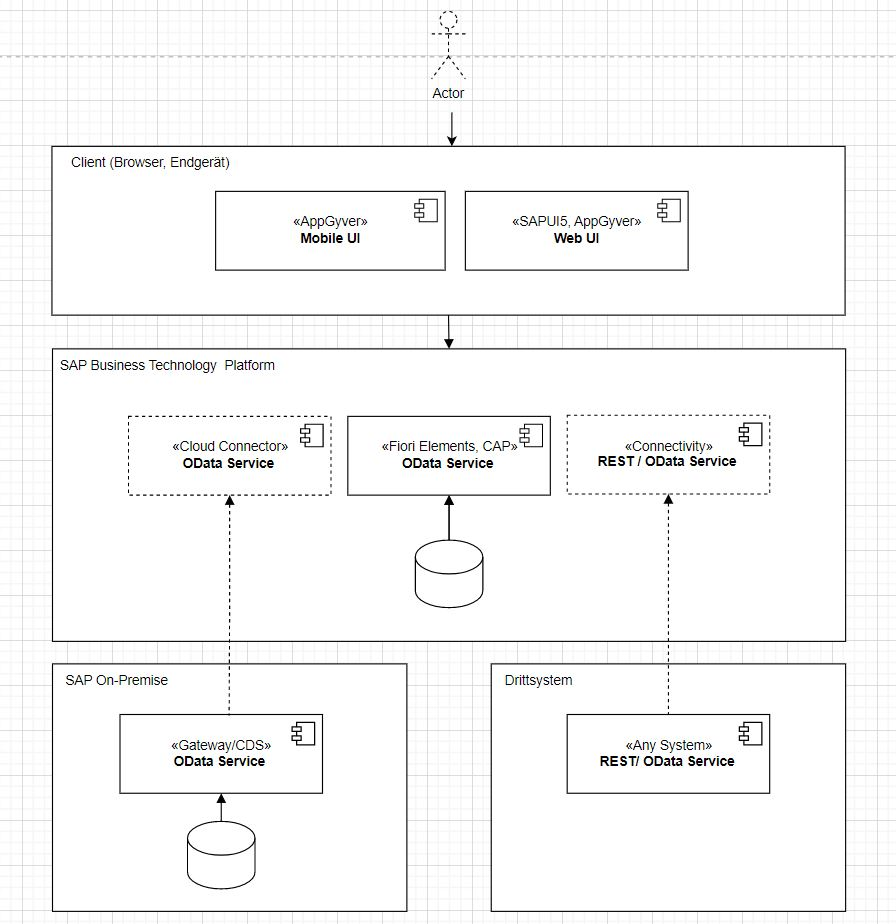
\includegraphics[width=0.8\textwidth]{Bilder/architecture/SAP_Anwendung_Architektur.jpg}
 \caption{Architektur einer SAP-Anwendung in der SAP BTP}
\end{figure}


\section{SAP Fiori}

SAP Fiori wurde von der SAP als visuelle Leitlinie eingeführt, um User Interfaces über unterschiedliche Anwendungen hinweg zu standardisieren. Hinter dem Begriff verbergen sich jedoch ebenfalls technologische Aspekte, wie beispielsweise SAP Fiori Elements.

Das Grundkonzept von SAP Fiori ist es, Benutzeroberflächen so zu gestalten, dass Nutzer von Geschäftsanwendungen in ihrer täglichen Arbeit bestmöglich unterstützt werden, unabhängig davon, welche Endgeräte sie benutzen. Im Mittelpunkt stehen dabei Themen wie Usability, die Haptik und die User Experience der Anwendungen und folgende Grundsätze \cite[S.31]{fiori}:

\begin{itemize}[noitemsep]
\item Eine SAP-Fiori-App stellt dem Anwender nur die Funktionen zur Verfügung, die seiner Rolle entsprechen, sodass er nicht durch irrelevante Optionen abgelenkt wird.
\item Mit SAP Fiori können Anwender sowohl auf mobilen Geräten als auch auf PCs arbeiten, wobei die Fiori-Anwendungen an das jeweilige Gerät angepasst werden müssen.
\item SAP-Fiori-App statten exakt die Funktionen des Anwendungsfalles aus. Die Funktionen, die nicht für Abarbeiten des Anwendungsfalles erforderlich sind, werden nicht in die Fiori-App ausgerichtet.
\item SAP Fiori folgt einer einheitlichen Interaktion Designsprache und verfügt über ein standardisiertes Oberflächendesign.
\item Die wesentlichen Funktionen der Fiori-Apps sollten für den Anwender intuitive bedienbar sein. Die Fiori-Apps sollen auch ansprechend sein \cite[S.34-35]{fiori}.
\end{itemize}

Der Fokus auf spezialisierte Applikationen macht es notwendig, diese zentral bereitzustellen. Das SAP Fiori Launchpad ist deswegen der zentrale Bereich, in welchem die SAP Fiori-Anwendungen zusammengeführt werden. Es stellt den Fiori-Apps Services wie Navigation und Anwendungskonfiguration zur Verfügung. Das Launchpad ist rollenbasiert und muss anwenderspezifisch angepasst werden. Die Rolle des Anwenders definiert somit, welche Fiori-App auf den Launchpad angezeigt werden \cite{sap:fiorilp}.

SAP Fiori als Design-Richtlinie wird im weiteren Verlauf nicht weiter betrachtet. Die Grundsätze finden sich jedoch in SAP Fiori Elements und auch in SAPUI5 wieder.

\section{SAP AppGyver }
\subsection{Grundlage von AppGyver}

AppGyver ist ein Pionier in der LCNC-Entwicklung. Das Unternehmen mit Hauptsitz in Helsinki wurde im Jahr 2010 gegründet und hat seit Gründung den Fokus auf der LCNC-Entwicklung \cite{sap:lcnc}. Mit Composer Pro stellt AppGyver eine zentrale Entwicklungsumgebung bereit, um Anwendungen für unterschiedliche Geschäftsprozesse und Anwendungsszenarien zu entwickeln, ohne eigenen Code zu schreiben. Diese Anwendungen können nicht nur als Webanwendungen, sondern auch als mobile Anwendungen eingesetzt werden. AppGyver unterstützt sowohl iOS mit Bereitstellung der Anwendungen im App Store als auch Android Phone mit Bereitstellung in Google Play. 

Im Februar 2021 wurde AppGyver von SAP übernommen und seitdem gibt es 2 Editionen: die Community Edition und die SAP Enterprise Edition. Die Community Edition basiert auf der initialen Version von AppGyver und bleibt zunächst unabhängig von SAP. Die Benutzer können es weiterhin kostenlos nutzen. Die SAP Enterprise Edition dagegen wird in das SAP-Ökosystem integriert und ist Bestandteil der SAP BTP. Zu den zusätzlichen Funktionen der Enterprise-Version zählen: 
 
\begin{itemize}[noitemsep]
\item Integration mit der SAP BTP Authentifizierung für Webanwendungen direkt in AppGyver.
\item Erweiterte Integration von Daten aus anderen SAP-Systemen.
\item Neue Enterprise-Funktionen, wie beispielsweise die Einführung einer Übersetzungsvariablen.
\item Nutzer können das Projekt in Echtzeit mit anderen teilen
\end{itemize}

Am 15. November 2022, während der Anfertigung dieser Arbeit, erfolgte ein Rebranding von SAP AppGyver in SAP Build Apps. Zudem wird das Tool in Zukunft Teil einer Suite an Applikationen unter dem Label SAP Build sein, welche den Fokus auf die gesamtheitliche LCNC-Entwicklung von Anwendungen, die Automatisierung von Prozessen sowie das Design von Unternehmenswebsites legt. Neben SAP Build Apps sind auch Build Process Automation und Build Work Zone in SAP Build enthalten \cite{sap:lcnc}. Neben der reinen Integration, wird SAP Build App zudem in Zukunft um neue Funktionen erweitert, wie beispielsweise "Visual Cloud Functions", die die Speicherung von Daten in der Cloud und die Ausführung von Geschäftslogik ermöglichen \cite{appgyver:coman}. Diese Erweiterungen werden jedoch im Rahmen dieser Thesis nicht weiter betrachtet.

\subsection{Entwicklungsumgebung: Composer Pro}
Eine Entwicklungsumgebung ist eine Zusammenstellung von Funktionen und Werkzeugen, die zur Entwicklung einer Anwendung notwendig sind. Werden diese gesamtheitlich und zentralisiert (via Internet) bereitgestellt, dann spricht man auch von einer Entwicklungsplattform. Composer Pro ist die zentrale Entwicklungsplattform von AppGyver. Dabei handelt es sich um eine spezialisierte LCNC-Plattform, mit der Anwendungen visuell und ohne Programmierung erstellt werden können. Der Aufbau der Plattform und die Funktionen sind dabei an die Zielgruppe, Citizen Developer ohne Programmiererfahrung, angepasst. Dennoch ist ein Verständnis des grundlegenden Aufbaus der Umgebung, sowie der Prinzipien zur Entwicklung einer Anwendung notwendig.

\begin{figure}[htbp]
 \centering
 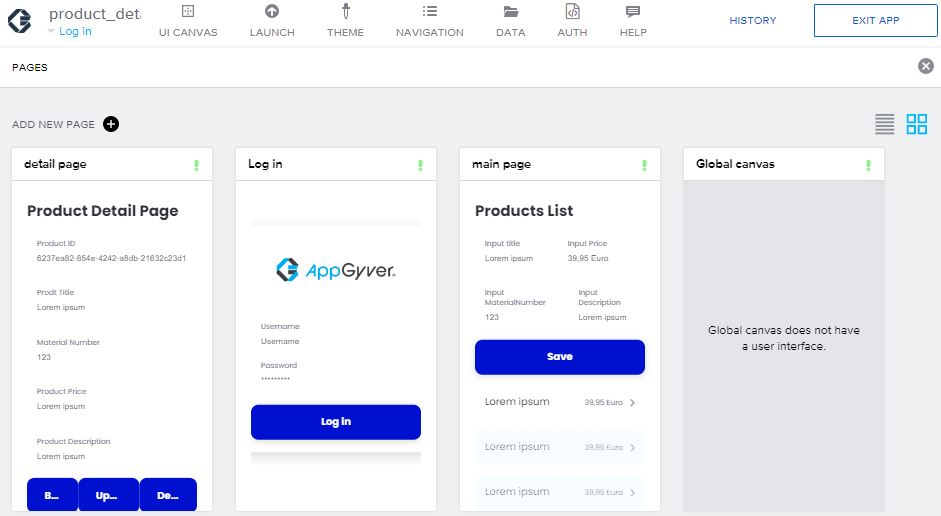
\includegraphics[width=0.9\textwidth]{Bilder/appgyver/2_2_Pages_in_AppGyver.jpg}
 \caption{Pages einer AppGyver-Anwendung}
\end{figure}

Eine Anwendung in AppGyver ist grundsätzlich in mehrere Pages unterteilt. Jede Page besitzt einen eigenen Canvas, auf dem weitere Inhalte platziert werden können. Am oberen Rand der Benutzeroberfläche befindet sich die zentrale Toolbar, über die der Entwickler auf alle Ressourcen und Werkzeuge von AppGyver zugreifen kann. 

\begin{figure}[htbp]
 \centering
 
\includegraphics[width=0.7\textwidth]{Bilder/appgyver/2_3_AppGyver Toolbar.JPG}
 \caption{Toolbar in Composer Pro}
\end{figure}

Dem LCNC-Ansatz folgend, finden sich in AppGyver keine programmatischen Bausteine (Code-Files, Klassen, etc.), sondern die diversen Funktionalitäten sind in eigenen, proprietären, Strukturen abgelegt. Dabei lassen sich diese grob in die Schichten des MVC-Models einteilen. Das MVC-Paradigma strukturiert die Implementierung einer Anwendung in folgende drei Schichten: 
\begin{itemize}[noitemsep]
\item \textbf{M} steht für Model und repräsentiert das Datenmodell. Das Datenmodell stellt die relevanten Daten bereit.
\item \textbf{V} bezieht sich auf View, d.h. die Präsentation. Diese Schicht ist zuständig für die Darstellung auf den Endgeräten und die Realisierung der Benutzerinteraktionen.
\item \textbf{C} steht für Controller, also die Steuerung. Controller steuern und verwalten die Views. Der Controller kommuniziert mit dem Modell, wenn eine Benutzeraktion mit einer Datenänderung stattfindet.
\end{itemize}

\begin{table}[!htbp]
  \centering
	\begin{tabular}{|l|l|} 
	\hline 
         \rowcolor{mygrey2} Applikations-Schicht&AppGyver-Baustein\\
	\hline  
	View&Page; View Component; Properties; Theme\\
	\hline
	Controller&Logic Flows; Formula Functions\\
	\hline
	Model&(Data) Variables; Data Resource\\
	\hline
	\end{tabular}
  \caption{AppGyver-Baustein in die Schichten des MVC-Models} 
\end{table}

\large{\textbf{View}}  \\
Eine Anwendung in SAP AppGyver besteht aus mehreren Pages, d.h. mehreren eigenen Sichten. Diese werden aus vorgefertigten und konfigurierten View Components zusammengesetzt. Der Komponentenbibliothek in Composer Pro bietet einen Überblick über alle verfügbaren Komponenten. Diese sind in drei Registerkarten unterteilt. Unter CORE sind die Kernkomponenten verfügbar, die in den meisten Anwendungen verwendet werden. Dies sind beispielsweise Texte, Buttons oder Input-Felder. Unter BY ME sind die Komponenten aufgelistet, die der Entwickler selbst für diese Anwendung erstellt hat. Komponenten, die aus dem Marketplace für diese Anwendung hinzugefügt wurden, sind auf der Registerkarte \emph{INSTALLED} zu finden \cite{appgyver:vc}. Jede View Component besitzt spezifisch Eigenschaften (Properties), die sich in dem kontext-sensitiven Panels „Component Properties“ und „Style“ angepasst werden können. Der Layout-Tree, der sich unten in der rechten Seitenleiste befindet, zeigt die komplette Struktur der Komponenten in der Anwendung an und ermöglicht die direkte Auswahl. Weiterhin ist es möglich, einen grundlegenden Theme mit Styles bereitzustellen, der die grundlegenden Farben, Schriften, etc. für die Anwendung festlegt.

\begin{figure}[htbp]
 \centering
 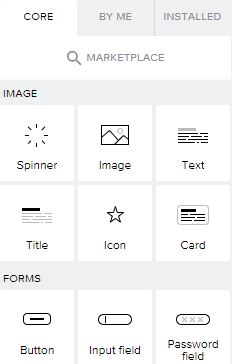
\includegraphics[width=0.3\textwidth]{Bilder/appgyver/2_4_Komponentenbibliothek.JPG}
 \caption{View-Components in Composer Pro}
\end{figure}

\large{\textbf{Model}} \\
AppGyver unterstützt in Bezug auf die Datenintegration zwei Szenarien: Es können Daten lokal im Projekt angelegt und abgespeichert werden. Diese Daten sind dann jedoch nur für die lokale Applikation gültig. Alternativ kann auf externe Datenendpunkte (REST, OData) zugegriffen werden. Die Daten werden dann über die externen Schnittstellen abgefragt und können in der Anwendung angezeigt werden. Zur Abbildung von Datenstrukturen und -flüssen gibt es in Composer Pro das Konzept der Variablen. Damit können ohne Programmierung verschiedene Arten von Strukturen festgelegt werden. „Page Variablen“ existieren nur für die aktuelle Seite und enthalten beliebige Werte, während „App Variablen“ über die gesamte Anwendung hinweg existieren. „Data Variablen“ befinden sich ebenfalls nur auf der aktuellen Seite und beinhalten die Funktion, interne und externe Datenstrukturen zu mappen. Diese Variablen können an die spezifischen Eigenschaften (Properties) einer View Component gebunden werden (Data-Binding) und stellen somit das Bindeglied zwischen Model und View dar. 

Weitere Variablen zur Ablage von Werten sind „Page Parameter“ (schreibgeschützte Textvariablen), die zur Übertragung von Daten zwischen den Seiten verwendet werden können und „Translation Variablen“, die für sprachabhängige Texte verwendet werden können.

\large{\textbf{Controller}} \\
Neben den Daten ist auch die Geschäftslogik ohne oder mit geringen Programmierkenntnissen umsetzbar. SAP AppGyver stellt hier Logische Ablauffunktionen bereit, mit denen per Drag\&Drop, sowie einer Konfiguration, komplexere Prozesse definiert werden können. Der Logic-Canvas befindet sich in der unteren Hälfte der Benutzeroberfläche. Für jede Komponente gibt es einen eigenen Logic-Canvas-Kontext, der eine spezifische Konfiguration erlaubt. Damit auf Nutzereingaben reagiert werden kann, stellen die View Components Events zur Verfügung. Diese werden immer dann geworfen, wenn eine spezifische Interaktion auftritt. 

Weiterhin existieren in AppGyver Formeln, die dazu genutzt werden können, um komplexere Logiken abzubilden. Dazu gibt es einen eigenen Formel-Editor, in dem die Logiken hinterlegt werden können. Tatsächlich stehen dort Formel-Typen zur Verfügung, die sich nahe an der richtigen Programmierung bewegen (Logische Operatoren, IF-Statements, etc) \cite{appgyver:logic}.

\begin{figure}[htbp]
 \centering
 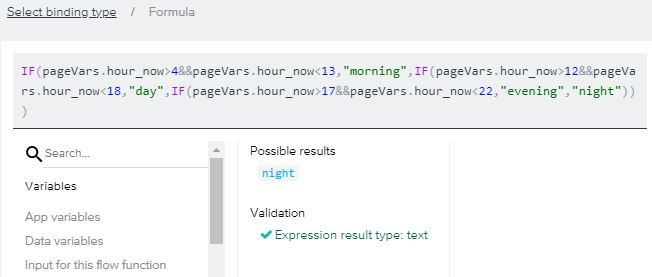
\includegraphics[width=0.8\textwidth]{Bilder/appgyver/2_5_Formula.jpg}
 \caption{Exemplarische Formel in AppGyver}
\end{figure} 

\section{SAPUI5}
\subsection{Grundlage von SAPUI5}
SAP Fiori beschreibt als Leitfaden die Entwicklungsrichtlinie zur Erstellung von Anwendungen im SAP-Umfeld. Für die Umsetzung sind jedoch auch technische Bausteine notwendig. Mit SAP WebDynpro, der vormals führenden UI-Technologie, ist SAP Fiori aber schwer umzusetzen, da der HTML-Code auf dem Server generiert und dann an das Endgerät übermittelt wird. In diesen Kontext ist die Entwicklung eines clientseitigen Ansatzes erforderlich. Bei einem clientseitigen Ansatz steht der Frontend-Server im Mittelpunkt der Kommunikation und lädt das UI-Framework, das die weiteren Verarbeitungsschritte übernimmt \cite[S.45-47]{fiori}.

SAPUI5 (kurz für: SAP UI Development Toolkit für HTML5) ist ein JavaScript-basiertes clientseitiges Framework und eine UI-Bibliothek, mit der SAP Fiori-Anwendungen sehr flexibel entwickelt und auf verschiedene Plattformen portiert werden können. Die SAPUI5-Bibliothek basiert auf modernen Web-Standards, wie JavaScript, HTML5 und CSS3 \cite[S.139]{sapui5}. SAPUI5 verfügt über mehr als 500 UI-Controls, die an den neuesten SAP Fiori Design Guidelines ausgerichtet sind, und bietet integrierte Unterstützung für Enterprise-Funktionen, wie Datenbindung, Routing, Message Handling, Mehrsprachigkeit, etc. Heute ist SAPUI5 der Standard für die Implementierung von Frontend-Anwendungen im SAP-Umfeld \cite{sap:ui5}.

Da es sich bei SAPUI5 nicht um eine LCNC-Technologie handelt, ist ein grundlegendes Programmierverständnis in der Sprache JavaScript notwendig. Zudem setzt SAPUI5 das Verständnis einiger Entwurfsmuster voraus. Das MVC-Paradigma beispielsweise strukturiert die Implementierung von SAPUI5-Anwendungen in drei Schichten, die sich so auch im Quellcode wiederfinden.

\begin{itemize}[noitemsep]
\item \textbf{Model:} Hier stehen spezielle Klassen zur Verfügung, die den Zugriff auf unterschiedliche Arten von Daten abstrahieren (JSONModel, ODataModel, XMLModel).
\item \textbf{View:} Die View beinhaltet den Aufbau des User Interfaces und SAPUI5 stellt hier UI Controls zur Verfügung, dafür genutzt werden. Diese lassen sich via JavaScript, HTML oder XML definieren und konfigurieren.
\item \textbf{Controller:} Zu jeder View gibt es in SAPUI5 einen Controller, der eine Benutzeraktion über Events und zugehörige Callback Implementierungen steuert, sowie komplexere Geschäftslogik enthalten kann \cite[S.149]{sapui5}.
\end{itemize}

Da es sich bei SAPUI5 um ein komplexeres Framework handelt, können an dieser Stelle nicht alle Facetten im Detail erklärt und beschrieben werden. In Kapitel 3.3 werden ihm Rahmen der Implementierung jedoch einige genutzte Dinge vorgestellt.

\subsection{Entwicklungsumgebung: Visual Studio Code}
Durch den freien Programmieransatz ist SAPUI5 nicht an eine Entwicklungsumgebung/plattform gebunden. Im Rahmen dieser Thesis wird Visual Studio Code (kurz: VS-Code) für die Umsetzung verwendet. VS-Code ist ein Quellcode-Editor von Microsoft, der im Jahr 2015 für verschiedene Betriebssysteme wie Windows, MacOS und Linux veröffentlicht wurde. Er unterstützt diverse Programmiersprachen und Frameworks (z.B. JavaScript, TypeScript und Node.js), kann jedoch über das Erweiterungskonzept um weitere Programmiersprachen, Laufzeiten und Funktionen ergänzt werden \cite{vsc:ov}. VS-Code ist heute aufgrund der ausgereiften Funktionen und der guten Bedienung ein Standard in der Entwicklung von Web-Anwendungen \cite{wiki:vsc} und wird deswegen an dieser Stelle potenziellen anderen Entwicklungsumgebungen vorgezogen.

Der Arbeitsbereich des VS-Code besteht aus ein oder mehreren Verzeichnissen. Es vereinfacht die sprachübergreifende Anwendungsentwicklung in einer integrierten Entwicklungsumgebung. VS-Code integriert ein voll funktionsfähiges Terminal mit dem Editor, um Shell Skript und Kommenden durchzuführen. Das integrierte Terminal kann verschiedene Shells verwenden, die auf dem Rechner installiert sind \cite{vsc:tb}.

Die lokale Implementierung der SAPUI5-Anwendung in VS-Code erfordert die zusätzliche Installation von weiteren Bibliotheken: das SAP Cloud Application Programming Model (kurz: SAP CAP) und des Easy UI5 Generators. Das SAP CAP ist ein Framework zur Erstellung von Backend-Anwendungen und kommt auch bei Fiori Elements zum Einsatz \cite{cap:ov}. Mit Hilfe von Core Data Services als die universelle Modellierungssprache für Domänenmodelle und Servicedefinitionen, können in sehr kurzer Zeit Datenmodelle generiert und als OData-Service bereitgestellt werden \cite{cap:ov}. Der Easy UI5 Generator enthält Vorlagen zur Erstellung einer SAPUI5-Anwendung mit aktuellen Best Practices. So lassen sich bereits die grundlegenden Strukturen einer Anwendung erstellen, auf deren Basis die Entwicklung dann stattfinden kann \cite{cap:geui5} 

Um die UI5-Anwendung zu implementieren, muss die Entwicklungsumgebung wie folgt eingerichtet werden:
\begin{itemize}[noitemsep]
\item Herunterladen und Installieren des aktuellen Node.js Installationspakets von https://nodejs.org/en/download/ inklusive Runtime und Package Manager (npm). Node.js bietet eine asynchrone, ereignisgesteuerte Laufzeitumgebung für Javascript und wird für das lokale Betreiben eines Webservers verwendet \cite{wiki:nodejs}.
\item Installieren von yeoman und dem Easy-ui5 Generator. Yeoman ist ein Kommandozeilen-Scaffolding-Tool für Node.js, um das Gerüst für die weitere Entwicklung der SAPUI5-Anwendung zu generieren 
\item Installieren der SAP Cloud Application Programming Model-Module (@sap/cds-dk und @sap/cds). 
\item Herunterladen und Installieren der SQLite-Datenbank-Treiber. Als ein leicht eingebettetes Datenbanksystem, lässt sich SQLite direkt in entsprechende Anwendungen integrieren, ohne keine weitere Server-Software \cite{wiki:sqlite}.
\item Installation der VS Code Erweiterungen für SAP Fiori und SAP CAP CDS, zur Unterstützung bei der Entwicklung.
\end{itemize}

Das cds-dk und SQLite werden benötigt, um bei der lokalen Entwicklung einen OData Mock Service zu erzeugen. Die VS-Code-Erweiterungen bieten Sprachunterstützung für die Core Data Services (CDS), welche die Grundlage des SAP Cloud Application Programming Model (CAP) bilden, sowie für SAPUI5 \cite{vsc:cdsext}.

\section{Fiori Elements}
\subsection{Grundlage von Fiori Elements}
SAP Fiori als gestalterische Richtlinie lässt sich mit SAPUI5 technisch umsetzen. Allerdings ist dort immer Programmieraufwand nötig. Als LCNC-Ansatz stellt die SAP jedoch mit Fiori Elements eine Technologie zur Verfügung, mit der UI Controls und sogar komplette Applikationen automatisch auf Basis von Metadaten zur Laufzeit generiert werden können. Die Metadaten werden dabei via OData-Annotationen beschrieben, die vom Backend-Service bereitgestellt werden müssen \cite[S.48]{fiori}. SAP Fiori Elements basiert technologisch auf SAPUI5 und erweitert dieses um intelligente Komponenten und Views. SAP Fiori Elements umfasst sogenannte Floorplans, d.h. Grundrisse und UI-Patterns für gängige Anwendungsfälle. Fiori Elements verfügt über die folgenden vier grundlegenden Floorplans:

\begin{itemize}[noitemsep]
\item List Report und Object Page
\end{itemize}

Ein List Report wird verwendet, wenn Elemente in einer Tabelle oder Liste dargestellt werden sollen. Mit dem List Report können die Objekte angezeigt, gefiltert und bearbeitet werden. Der List Report wird in der Regel in Verbindung mit der Objekt Page verwendet. Auf die Objekt Page kann der Nutzer durch Klicken auf ein einzelnes Element in der Liste gelangen und dort detaillierte Informationen über einzelne Objekte angezeigt bekommen und es bearbeiten.

\begin{figure}[htbp]
 \centering
 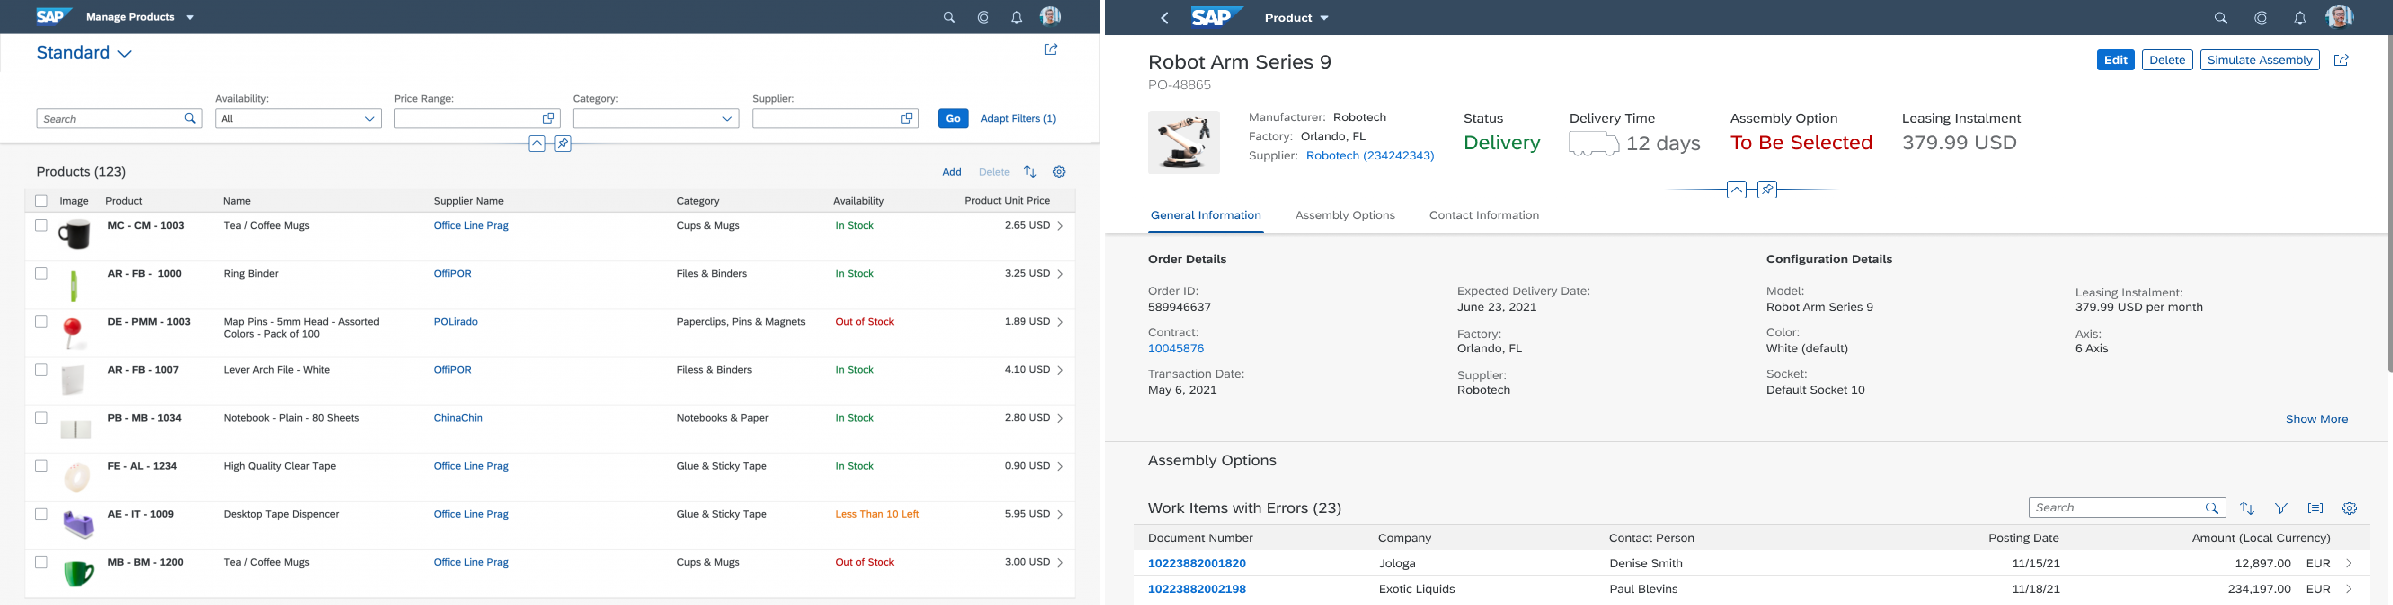
\includegraphics[width=1.0\textwidth]{Bilder/fiori_element/list_object_page.png}
 \caption{List Report und Object Page (Quelle: SAP Fiori Design Guidelines. URL: https://experience.sap.com/fiori-design-web/smart-templates)}
\end{figure} 

\begin{itemize}[noitemsep]
\item Worklist
\end{itemize}

Eine Worklist zeigt ebenfalls eine Liste von Elementen an, die von Benutzer bearbeitet werden sollen. In einer Worklist ist jedoch keine komplexe Filterung möglich und die Anzeige, bzw. das Editieren erfolgt ausschließlich in der Worklist-Ansicht \cite{sap:ufef}.

\begin{itemize}[noitemsep]
\item Overview Page
\end{itemize}

Ein Overview Page ermöglicht es, den Nutzern eine große Menge unterschiedlicher Informationen für einen Überblick bereitzustellen. Unterschiedliche Informationen werden in verschiedenen Cards visualisiert. Eine Card zeigt die Details zu einem bestimmten Geschäftsobjekt. Mit der Overview Page können Anzeigen, Filtern und Verarbeiten von Daten einfach und effizient gemacht werden.

\begin{figure}[htbp]
 \centering
 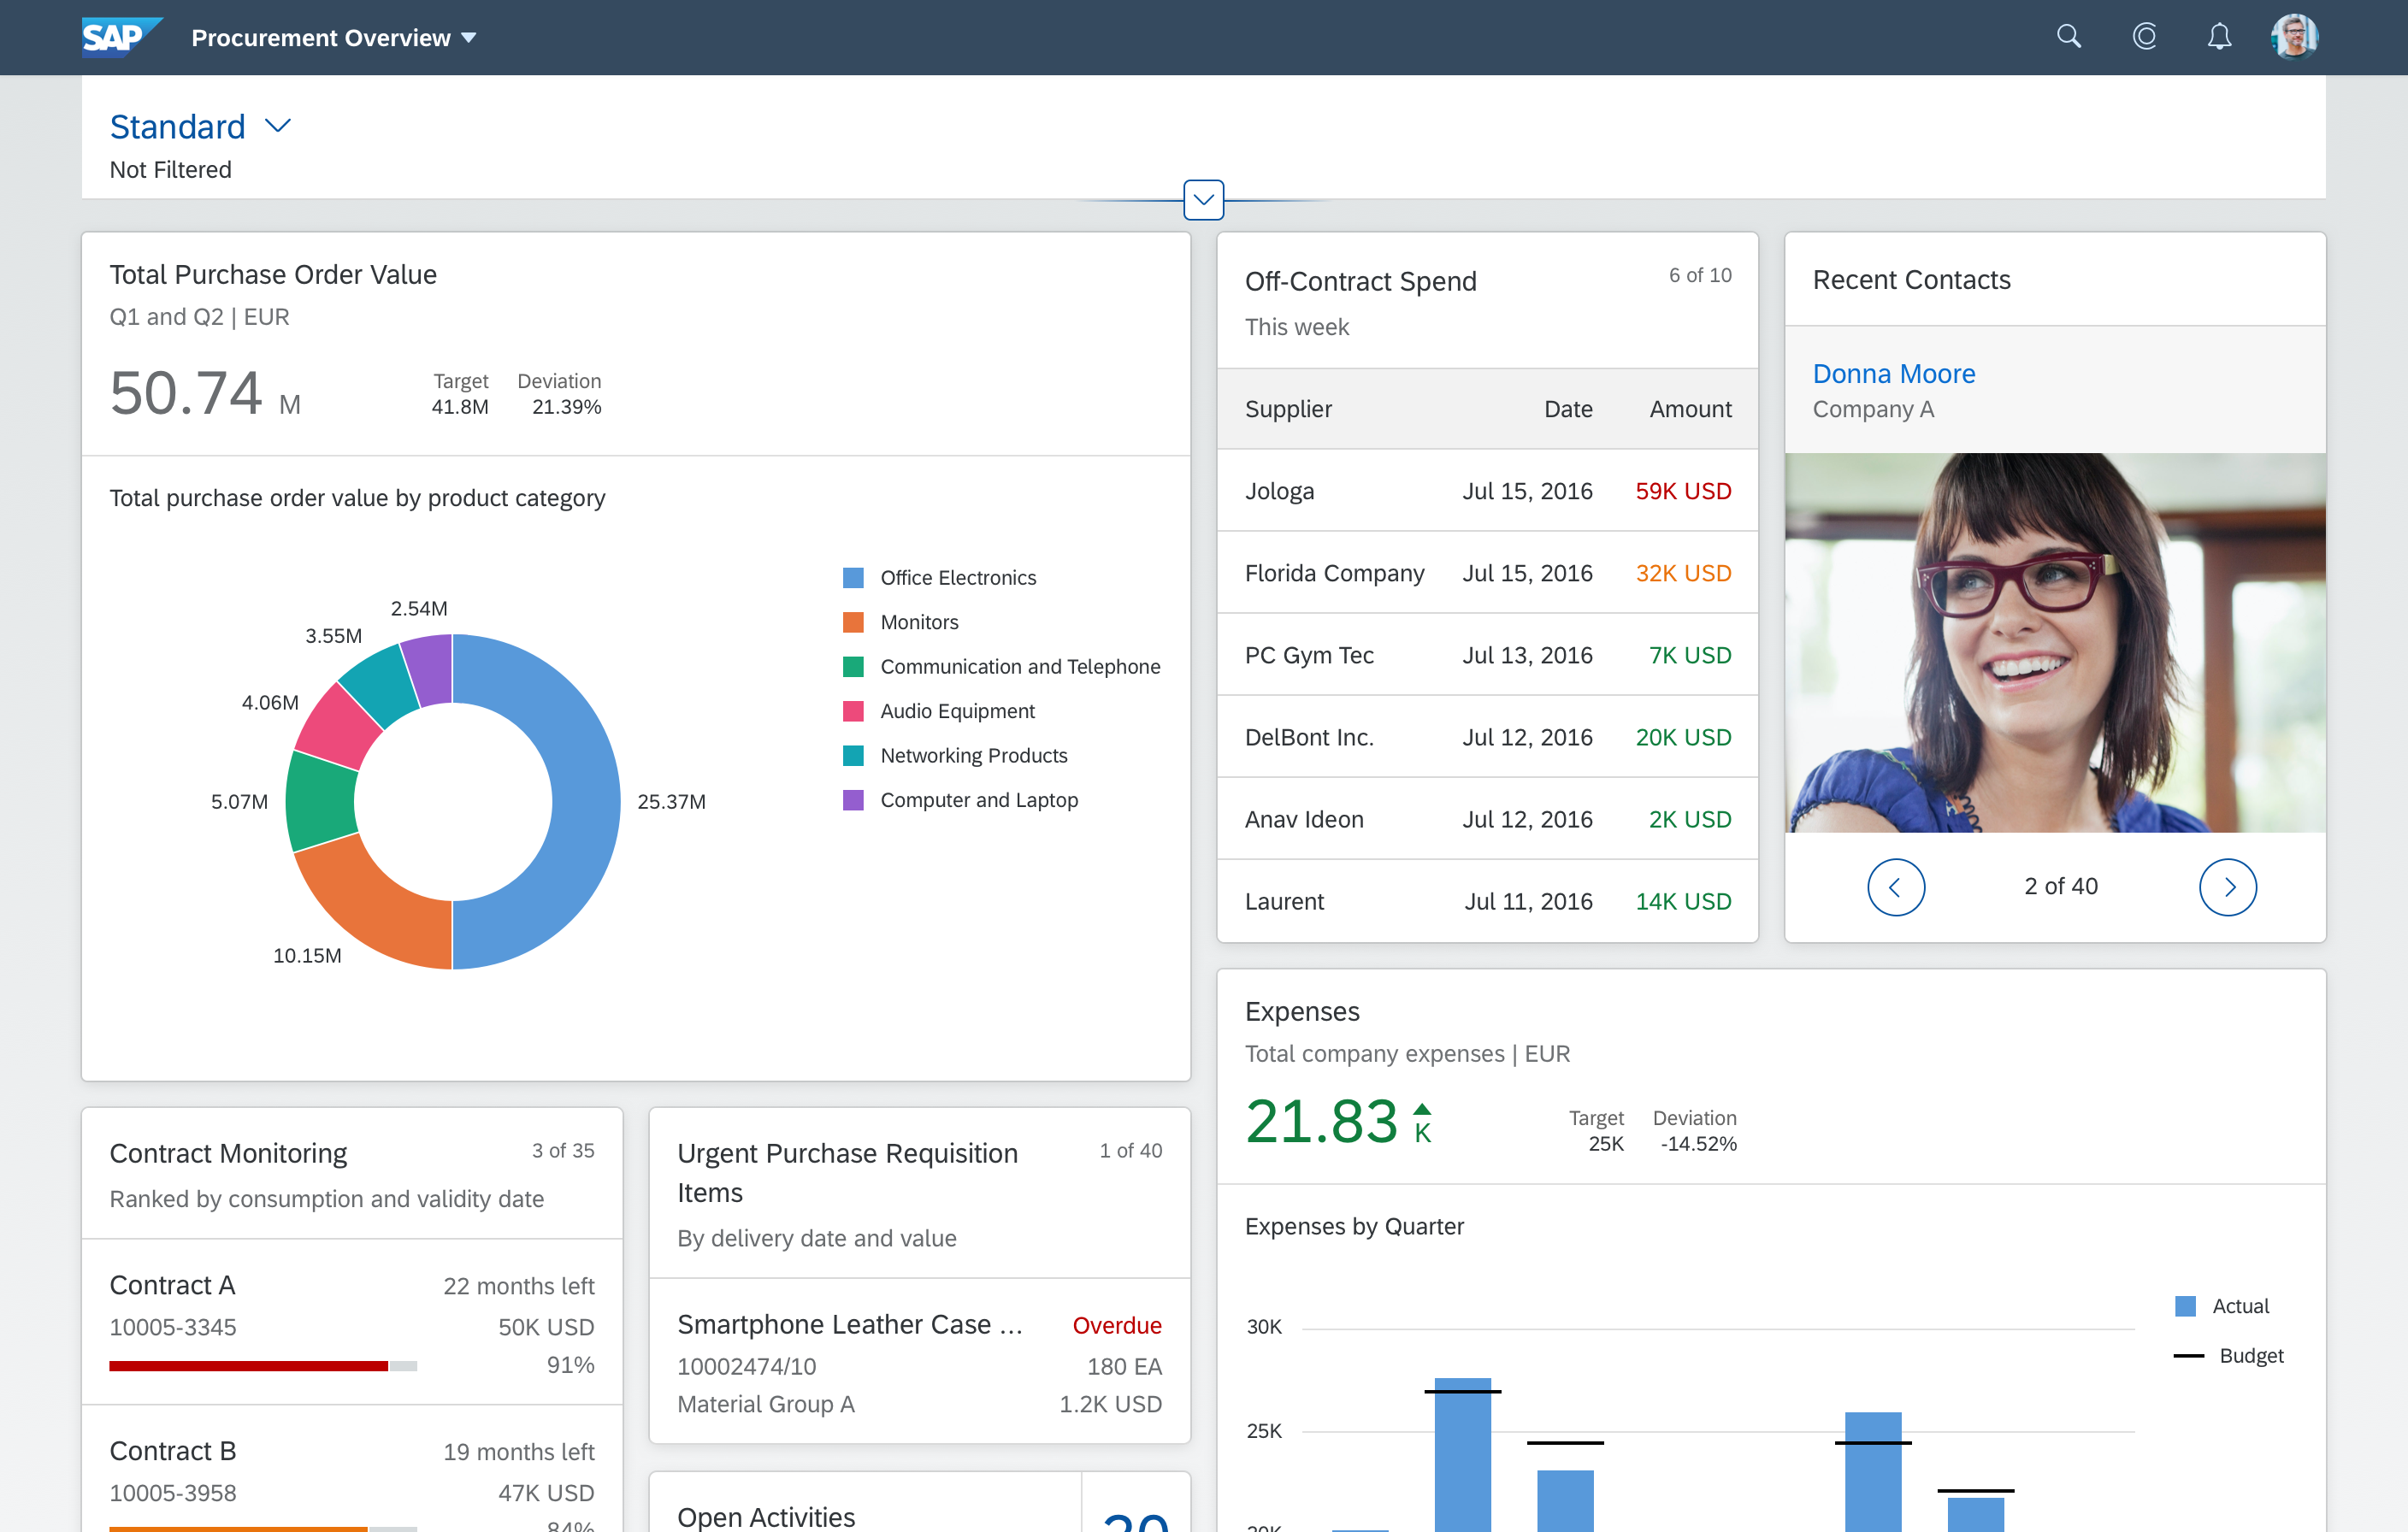
\includegraphics[width=0.6\textwidth]{Bilder/fiori_element/Overview-page.png}
 \caption{Overview Page (Quelle: SAP Fiori Design Guidelines. URL: https://experience.sap.com/fiori-design-web/smart-templates)}
\end{figure} 

\begin{itemize}[noitemsep]
\item Analytical List Page
\end{itemize}

Die Analytical List Page ist die Weiterentwicklung von List Report und verfügt über mehr Funktionen: Daten können in verschiedene Perspektiven analysiert werden, z.B. durch Drill-Downs zur Ursachenforschung \cite{sap:ufef}.

Mit Hilfe von Extension Points in den Floor-Plans können in einer Fiori Element-Anwendung zusätzliche Funktionalitäten hinzugefügt werden. Dafür ist jedoch immer eine Programmierung erforderlich.
SAP Fiori Elements ohne Extensions benötigt keinen Programmieraufwand, setzt jedoch einen OData-Service und eine Konfiguration der Annotationen voraus. Hierfür stehen potentiell unterschiedliche Technologien zur Verfügung. Dank der SAP eigenen Entwicklungsumgebung, SAP Business Application Studio, können jedoch komplette SAP Fiori Elements-Anwendungen inklusive der Defintion von Datenstrukturen und OData-Services und Annotationen visuell aufgebaut werden \cite{sap:dafe}.



\subsection{Entwicklungsumgebung: Business Application Studio} 
Grundsätzlich kann SAP Fiori Elements mit verschiedenen Entwicklungsumgebungen erstellt werden. Durch die sehr gute Integration und Bereitstellung einer LCNC-Umgebung, eignet sich das SAP Business Application Studio (BAS) jedoch sehr gut für das Erstellen einer Anwendung im Kontext dieser Thesis. BAS ist ein Service der SAP Business Technology Platform (SAP BTP), der seit Februar 2020 als Nachfolger der SAP Web IDE zur Verfügung steht. SAP BAS ist ein Cloud-basiertes Werkzeug, das nicht lokal installiert werden kann und im Browser des Nutzers ausgeführt wird und entspricht damit den Kriterien einer Entwicklungsplattform \cite{btp:ov}.

Das Business Application Studio lässt sich via Dev Spaces für unterschiedliche Anwendungsarten konfigurieren. Die Entwicklungsszenarien umfassen zum Beispiel SAP Fiori, SAP S/4HANA Erweiterungen, Workflows und SAP HANA-Anwendungen. In jedem Dev Space werden je nach Auswahl eine Reihe von vordefinierten Erweiterungen installiert, die spezialisierte Funktionen bereitstellen \cite{btp:ov}.

Neben der klassischen Code-basierten Entwicklung, stellt BAS auch die Möglichkeit bereit, „Low-Code basierte Full-Stack Anwendungen“ zu entwickeln. Dafür sind dann diverse Wizards und UI-Masken vorhanden, die im Hintergrund automatisch den notwendigen Quellcode interpretieren und erstellen. Eine Full-Stack-Anwendung besteht dabei aus dem Datenmodell und OData-Service des SAP Cloud Application Programming Models und SAP Fiori Elements als Frontend-Technologie. Alle notwendigen Parameter lassen sich via UI konfigurieren.

Im Rahmen dieser Arbeit wird ein Dev Space erstellt, der als Entwicklungsumgebung für die Low-Code-basierte Full-Stack-Anwendung ausgewählt wurde, um den in Kapitel 1, Abschnitt 1.3 beschriebenen Anwendungsfall mit Fiori-Elements zu entwickeln. 
